%\begin{frame}{Thoughts}
%    \begin{block}{Input}
%        \begin{itemize}
%            \item Different variable set $\rightarrow$ different problem topology
%            \item Concatenate layers as input $\rightarrow$ Combination of more information and final output
%            \item Separate background from the adversary's input $\rightarrow$ remove possible bias
%        \end{itemize}
%    \end{block}
%    %
%    \begin{block}{General}
%        \begin{itemize}
%            \item Different analysis $\rightarrow$ Insight on the network's general inability
%        \end{itemize}
%    \end{block}
%\end{frame}

\begin{frame}{Conclusions}
    \begin{block}{Network performance}
        \begin{itemize}
            \item Classic approach does not deliver expected results
            \item Changing the input results in slight improvements on the sensitivity
        \end{itemize}
    \end{block}
    %
    \begin{block}{Insights}
        \begin{itemize}
        	\item Classifier and adversary need to be trained as a combination
            \item The complex architecture of the adversary is not justified by just inputting the classifier's output
            \item Learning rate is a the central hyper-parameter for the loss behaviour
        \end{itemize}
    \end{block}
\end{frame}

\begin{frame}{}
    \begin{figure}
        \centering
        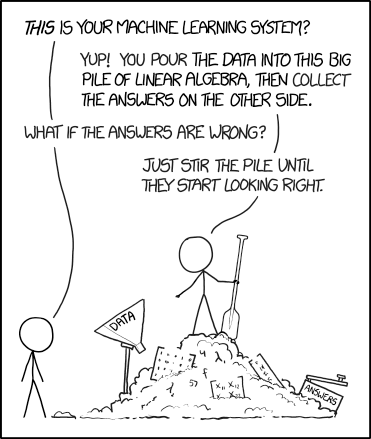
\includegraphics[width=0.4\textwidth]{xkcd}
        \caption{https://xkcd.com/1838/}
    \end{figure}
\end{frame}